\documentclass[a4paper,12pt]{article} % добавить leqno в [] для нумерации слева
\usepackage[a4paper,top=1.3cm,bottom=2cm,left=1.5cm,right=1.5cm,marginparwidth=0.75cm]{geometry}
%%% Работа с русским языком
\usepackage{cmap}					% поиск в PDF
\usepackage[warn]{mathtext} 		% русские буквы в фомулах
\usepackage[T2A]{fontenc}			% кодировка
\usepackage[utf8]{inputenc}			% кодировка исходного текста
\usepackage[english,russian]{babel}	% локализация и переносы
\usepackage{physics}
\usepackage{multirow}
\usepackage{float}
\usepackage{amsmath}
\usepackage{mathtext}
\usepackage[T1,T2a]{fontenc}
\usepackage[utf8]{inputenc}
\usepackage[english, bulgarian, russian]{babel}
\usepackage{pgfplots}
\usepackage[export]{adjustbox}
\usepackage{siunitx}
\usepackage{booktabs}
\usepackage{pgfplotstable}
\restylefloat{table}


\usepackage{graphicx}

\usepackage{wrapfig}
\usepackage{tabularx}

\usepackage{hyperref}
\usepackage[rgb]{xcolor}
\hypersetup{
colorlinks=true,urlcolor=blue
}

%%% Дополнительная работа с математикой
\usepackage{amsmath,amsfonts,amssymb,amsthm,mathtools} % AMS
\usepackage{icomma} % "Умная" запятая: $0,2$ --- число, $0, 2$ --- перечисление

%% Номера формул
\mathtoolsset{showonlyrefs=true} % Показывать номера только у тех формул, на которые есть \eqref{} в тексте.

%% Шрифты
\usepackage{euscript}	 % Шрифт Евклид
\usepackage{mathrsfs} % Красивый матшрифт

%% Свои команды
\DeclareMathOperator{\sgn}{\mathop{sgn}}

%% Перенос знаков в формулах (по Львовскому)
\newcommand*{\hm}[1]{#1\nobreak\discretionary{}
{\hbox{$\mathsurround=0pt #1$}}{}}

\date{\today}

\begin{document}

\begin{titlepage}

	\vspace*{10cm}
	{\huge
		\begin{center}
			{\bf
            Отчёт о выполнении лабораторной работы 1.2.5}\\
			Изучение вынужденной регулярной прецессии гироскопа
		\end{center}
	}
	\vspace{8cm}
	\begin{flushright}
		{\LARGE\\ Трунов Владимир \\
			\vspace{0.2cm}
			Б01-103}
	\end{flushright}
	\vspace{8cm}
\end{titlepage}


\section{Аннотация}

В работе исследуется вынужденная прецессия гироскопа. Устанавливается зависимость скорости вынужденной прецессии от величины момента сил, действующих на ось гироскопа. Определяется скорость вращения ротора гироскопа и сравнивается со скоростью, рассчитанной по скорости прецессии. 


\section{Теоретические сведения}

Так как уравнения движения твердого тела можно записать в виде. 

\begin{center}

  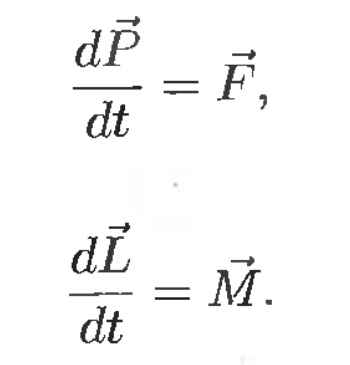
\includegraphics[width=0.2\linewidth]{IMG_1.jpg}\\
 
 \end{center}


Этих двух уравнений достаточно для полного описания состояния его движения. 

Так как если сила не зависит от угловой скорости, а момент -- от скорости поступательного движения, то эти уравнения можно рассматривать независимо друг от друга. 
Момент импульса твердого тела в его главных осях x, y, z равен

\begin{center}

  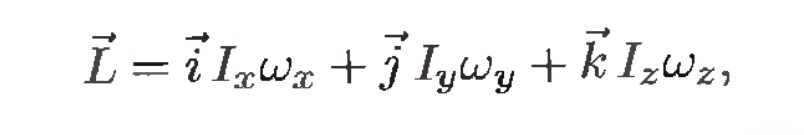
\includegraphics[width=0.4\linewidth]{IMG_2.jpg}\\
 
 \end{center}

Под действием момента внешних сил ось гироскопа медленно вращается вокруг оси у с угловой скоростью $\Omega$. Для гироскопа  массой $M_г$, у которого ось собственного вращения наклонена на углол $\alpha$ от вертикали, скорость прецессии, происходящей вокруг вертикальной оси под действием силы тяжести, равна. 

\begin{center}
  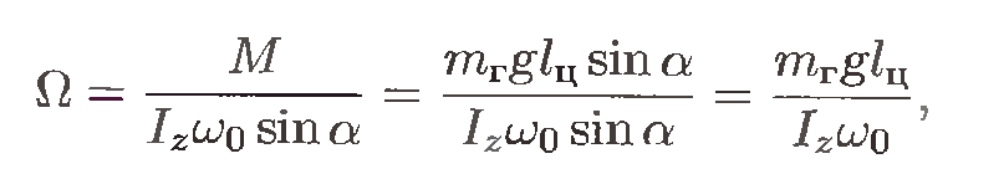
\includegraphics[width=0.4\linewidth]{IMG_3.jpg}\\
 
 \end{center}

\begin{center}

  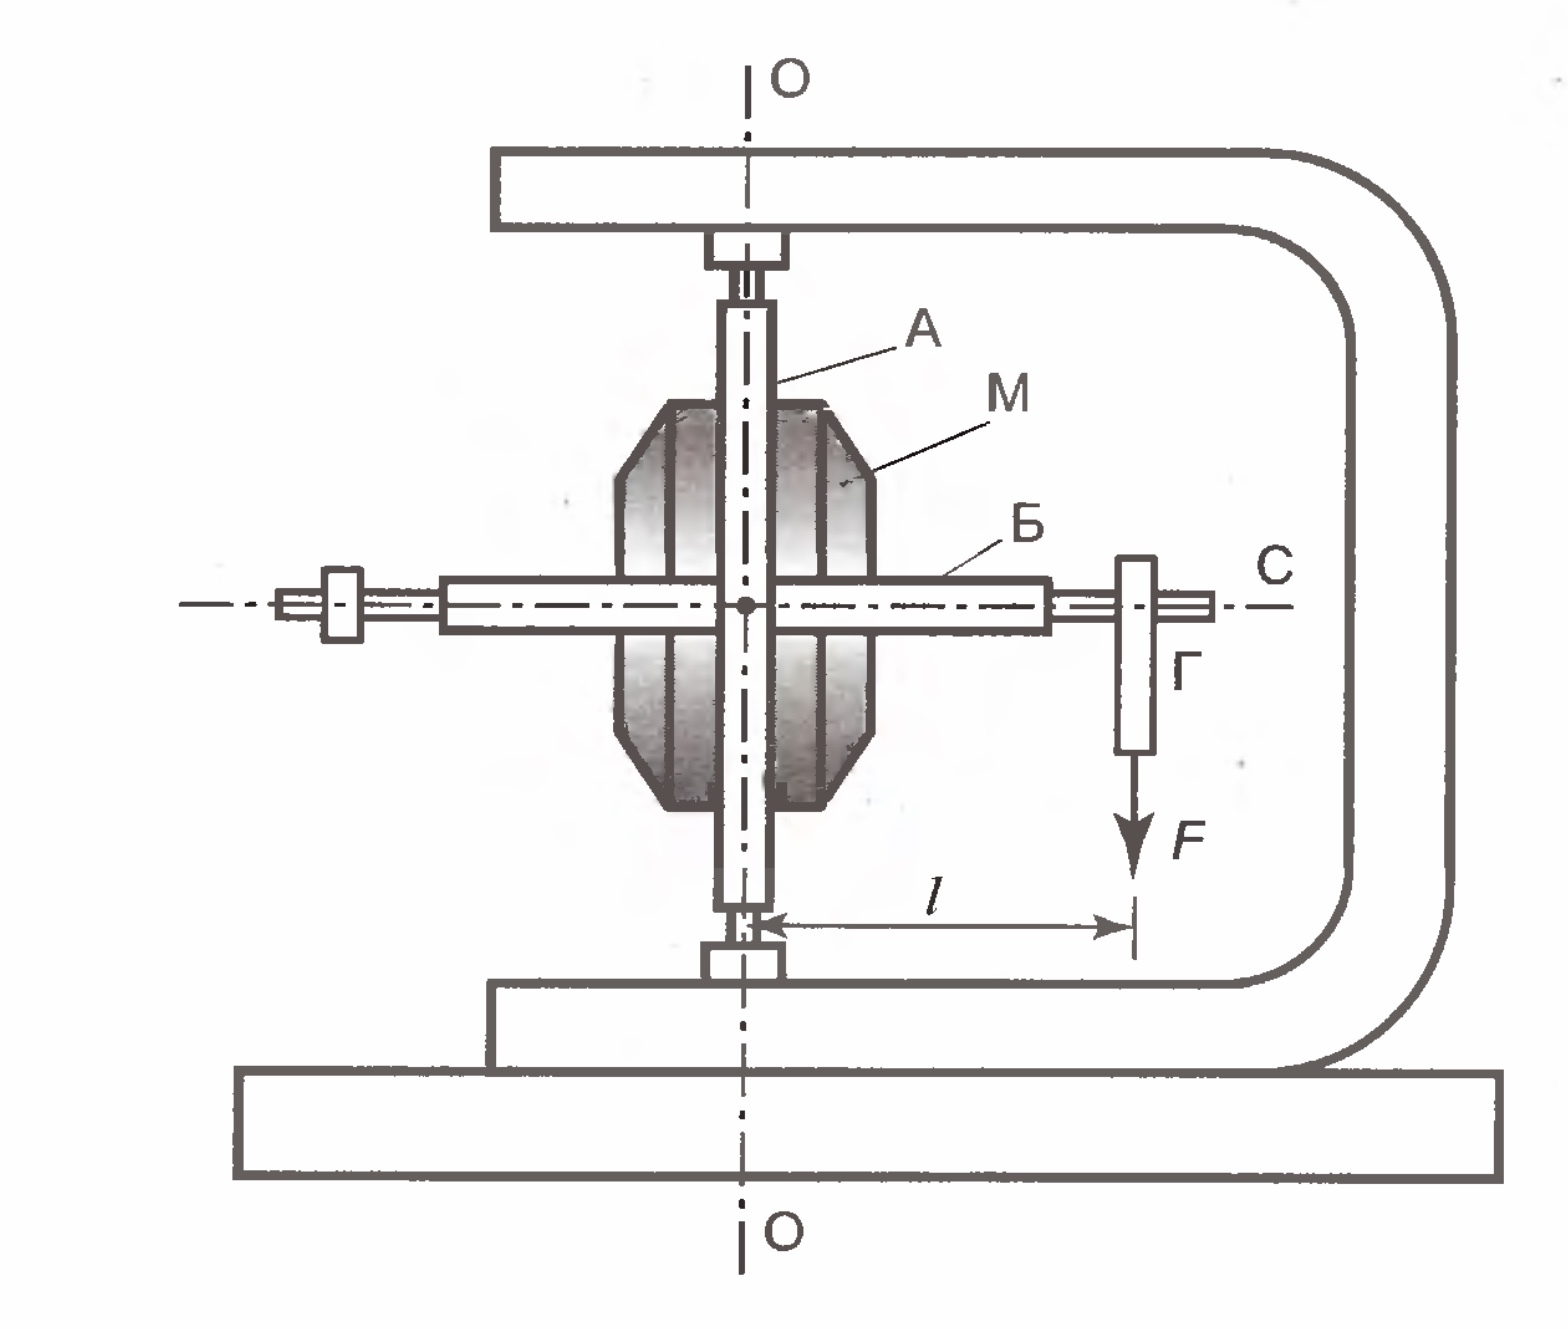
\includegraphics[width=0.5\linewidth]{IMG_4.jpg}\\
 
  Схема экспериментальной установки\\
 
 \end{center}

В данной работе исследуется регулярная прецессия уравновешенного гироскопа. 
Измерение скорости прецессии гироскопа позволяет вычислить угловую скорость вращения его ротора. 

\section{Оборудование и инструментальные погрешности}

В работе используются: гироскоп в кардановом подвесе, секундомер, набор грузов, отдельный ротор гироскопа, цилиндр известной массы, крутильный маятник, штангенциркуль, линейка.\\
\\
1. Точность измерения с помощью штангенциркуля -- 0,1 мм. \\
2. Точность измерения с помощью линейки -- 0,5 мм. \\
3. Точность измерения времени -- 0,2 с. \\
4. Точность измерения угла поворота гироскопа вокруг своей оси -- 3 градуса. \\
5. Точность измерения угла поворота во время опускания рычага -- 3 градуса. \\
\section{Результаты измерений и обработка данных}
\subsection{Подготовка к эксперименту}
Установим ось гироскопа в горизонтальное положение, осторожно поворачивая ее за рычаг С.
Включим питание гироскопа и подождем несколько минут, чтобы вращение ротора успело стабилизироваться.
Убедимся в том, что ротор вращается достаточно быстро: при легком постукивании по рычагу С последний не изменяет своего положения в пространстве.

Ротор вращается против часовой стрелки. 

При подвешивании к рычагу груза начинается прецессия гироскопа, а трение в горизонтальной оси приводит к тому, что рычаг начинает медленно опускаться.

\subsection{Измерение момента инерции ротора относительно оси симметрии $I_0$}
Повесим ротор, извлеченный из такого же гироскопа, к концу висящей проволоки так, чтобы ось симметрии гироскопа была вертикальна, и измерим период крутильных колебаний получившегося маятника.

\begin{align*}
  30T_0 =  97,0 \pm 0,5 \ c && T_0 = 3,23 \pm 0,02 \ c\\
\end{align*}
Заменим ротор гироскопа цилиндром, для которого известны данные:
\begin{align*}
  m &= 1617,8 \pm 0,1 \ г & d = 7,8 \pm 0,1 \ см\\
\end{align*}
Где m, h и d -- масса, высота и диаметр цилиндра соответственно.
И проведем аналогичное измерение для цилиндра:
\begin{align*}
  30T_1 =  118,7 \pm \ 0,5 \ c && T_1 = 3,96 \pm 0,02 \ c\\
\end{align*}


Так как момент инерции цилиндра относительно оси симметрии равен:

\begin{align*}
  I_1 &= \frac{md^2}{8} & I_1 = (1,23 \pm 0,03) \cdot 10^{-3} кг \cdot м^2 \\
\end{align*}

Тогда исходя из формулы вычислим момент инерции ротора $I_2$

\begin{align*}
  I_0 &= I_1 \frac{T_0^2}{T_1^2} & I_0 = (0,82 \pm 0,05) \cdot 10^{-3} кг \cdot м^2 \\
\end{align*}

\subsection{Определение частоты вращения ротора гироскопа}

Для определения частоты вращения ротора гироскопа будем исследовать зависимость скорости прецессии гироскопа в зависимости от момента силы, действующей на его ось. Результаты измерений представлены в таблице 1.

% Please add the following required packages to your document preamble:
% \usepackage{multirow}
\begin{table}[H]
	\centering
	\begin{tabular}{|c|c|c|c|c|c|c|c|c|c|c|c|c|c|c|c|c|c|}
		\hline
		№  & $ m $, кг          & $ l $, м            & $ M $, Н$\cdot$м      & $ \sigma_M $, Н$\cdot$м             & $ t $, с & $ N_\text{об} $ & $ T $, с & $ \langle T \rangle $, с   & $ \sigma_T $, с          &  $ \varepsilon_T, \%$   & $ \Omega $, $ \text{с}^{-1} $ & $ \sigma_\Omega $, $ \text{с}^{-1} $ \\ \hline
	1  & \multirow{3}{*}{0,336} & \multirow{3}{*}{0,122} & \multirow{3}{*}{0,402} & \multirow{3}{*}{0,004} & 425,95            & 14             & 30,43              & \multirow{3}{*}{30,43} & \multirow{3}{*}{0,04} & \multirow{3}{*}{0,12}  & \multirow{3}{*}{0,2065}                   & \multirow{3}{*}{0,0003} \\ \cline{1-1} \cline{6-8}
	2  &                        &                        &                        &                        & 426,23            & 14             & 30,45              &                        &                       &                        &                                           &                         \\ \cline{1-1} \cline{6-8}
	3  &                        &                        &                        &                        & 425,76            & 14             & 30,41              &                        &                       &                        &                                           &                         \\ \hline \hline
	4  & \multirow{3}{*}{0,269} & \multirow{3}{*}{0,122} & \multirow{3}{*}{0,322} & \multirow{3}{*}{0,003} & 264,57            & 7              & 37,80              & \multirow{3}{*}{37,87} & \multirow{3}{*}{0,08} & \multirow{3}{*}{0,21}  & \multirow{3}{*}{0,1659}                   & \multirow{3}{*}{0,0004} \\ \cline{1-1} \cline{6-8}
	5  &                        &                        &                        &                        & 265,46            & 7              & 37,92              &                        &                       &                        &                                           &                         \\ \cline{1-1} \cline{6-8}
	6  &                        &                        &                        &                        & 265,24            & 7              & 37,89              &                        &                       &                        &                                           &                         \\ \hline \hline
	7  & \multirow{3}{*}{0,215} & \multirow{3}{*}{0,122} & \multirow{3}{*}{0,257} & \multirow{3}{*}{0,002} & 142,09            & 3              & 47,36              & \multirow{3}{*}{47,41} & \multirow{3}{*}{0,17} & \multirow{3}{*}{0,36}  & \multirow{3}{*}{0,1325}                   & \multirow{3}{*}{0,0005} \\ \cline{1-1} \cline{6-8}
	8  &                        &                        &                        &                        & 142,39            & 3              & 47,46              &                        &                       &                        &                                           &                         \\ \cline{1-1} \cline{6-8}
	9  &                        &                        &                        &                        & 142,23            & 3              & 47,41              &                        &                       &                        &                                           &                         \\ \hline \hline
	10 & \multirow{3}{*}{0,174} & \multirow{3}{*}{0,122} & \multirow{3}{*}{0,208} & \multirow{3}{*}{0,002} & 116,81            & 2              & 58,41              & \multirow{3}{*}{58,39} & \multirow{3}{*}{0,25} & \multirow{3}{*}{0,43}  & \multirow{3}{*}{0,1076}                   & \multirow{3}{*}{0,0005} \\ \cline{1-1} \cline{6-8}
	11 &                        &                        &                        &                        & 116,65            & 2              & 58,33              &                        &                       &                        &                                           &                         \\ \cline{1-1} \cline{6-8}
	12 &                        &                        &                        &                        & 116,85            & 2              & 58,43              &                        &                       &                        &                                           &                         \\ \hline \hline
	13 & \multirow{3}{*}{0,138} & \multirow{3}{*}{0,122} & \multirow{3}{*}{0,165} & \multirow{3}{*}{0,002} & 147,55            & 2              & 73,78              & \multirow{3}{*}{73,80} & \multirow{3}{*}{0,25} & \multirow{3}{*}{0,34}  & \multirow{3}{*}{0,0851}                   & \multirow{3}{*}{0,0003} \\ \cline{1-1} \cline{6-8}
	14 &                        &                        &                        &                        & 147,51            & 2              & 73,76               &                        &                       &                        &                                           &                         \\ \cline{1-1} \cline{6-8}
	15 &                        &                        &                        &                        & 147,76            & 2              & 73,88              &                        &                       &                        &                                           &                         \\ \hline
	\end{tabular}
	\caption{Результат измерения зависимости скорости прецессии от момента сил}
	\label{sk_pre}
\end{table}

Момент силы, действующей на ось ротора гироскопа можно вычислить по следующей формуле:

\begin{equation}
M = mgl.
\end{equation}
Тогда погрешность вычисления момента силы определяется следующим соотношением:

\begin{equation}
\sigma_M = M\sqrt{\left( \frac{\Delta_\text{вес}}{m} \right)^2 + \left( \frac{\Delta_\text{лин}}{l} \right)^2}
\end{equation}

Скорость прецессии гироскопа можно найти по формуле:

\begin{equation}
\Omega = \frac{2\pi}{T}.
\end{equation}
При этом погрешность вычисления скорости прецессии равна:
\begin{equation}
\sigma_\Omega = \Omega \varepsilon_T.
\end{equation}
Полученные результаты записываем в таблицу 1.

Согласно уравнению, зависимость скорости прецессии $ \Omega $ от момента сил $ M $ должна быть линейной:

\begin{equation}
\Omega = kM,
\end{equation}
где
\begin{equation}
k = \frac{1}{I_0\omega_0}.
\end{equation}

Значит зависимость можно аппроксимировать с помощью метода наименьших квадратов. Перенесём все необходимые данные в таблицу 2:

\begin{table}[H]
	\centering
	\begin{tabular}{|c|c|c|c|c|c|}
		\hline
		№             & 1  & 2  & 3  & 4  & 5  \\
		\hline \hline
		$ M $, Н$\cdot$м             & 0,402  & 0,322  & 0,257  & 0,208  & 0,165  \\ \hline
		$ \sigma_M $, Н$\cdot$м       & 0,004  & 0,003  & 0,002  & 0,002  & 0,002  \\ \hline
		$ \varepsilon_M, \% $  & 0,87   & 0,90   & 0,94   & 1,00   & 1,09   \\ \hline \hline
		$ \Omega, \text{ с}^{-1} $          & 0,2065 & 0,1659 & 0,1325 & 0,1076 & 0,0851 \\ \hline
		$ \sigma_\Omega, \text{ с}^{-1} $    & 0,0003 & 0,0004 & 0,0005 & 0,0005 & 0,0003 \\ \hline
		$ \varepsilon_\Omega, \% $ & 0,12   & 0,21   & 0,36   & 0,43   & 0,34   \\ \hline
	\end{tabular}
	\caption{Данные для аппроксимации зависимости}
	\label{mnk}
\end{table}

По полученным данным построим график зависимости. Он представлен на рисунке 2.

\begin{center}

    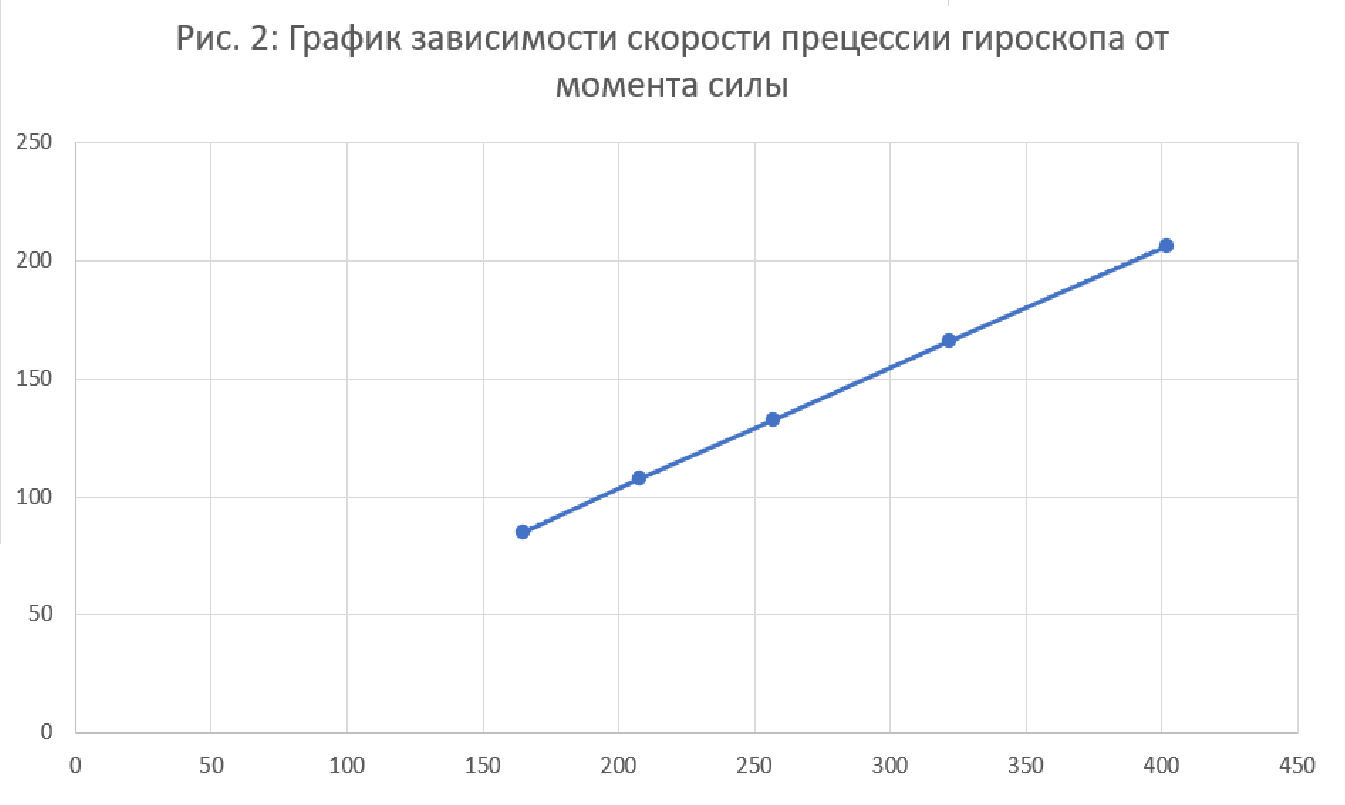
\includegraphics[width=1\linewidth]{omega.png}\\
   
   \end{center}

Коэффициент $ k $ можно вычислить по следующей формуле:\label{k}

\begin{equation}
k = \frac{\langle M\Omega\rangle}{\langle M^2 \rangle} \approx 0,5144 \text{ } \frac{1}{\text{Дж} \cdot \text{с}}.
\end{equation}
Случайную погрешность определения $ k $ можно вычислить по следующей формуле:

\begin{equation}
\sigma^\text{сл}_k = \frac{1}{\sqrt{N_\text{оп}-1}} \sqrt{\frac{\langle \Omega^2 \rangle}{\langle M^2 \rangle} - k^2} \approx 0,0005 \text{ } \frac{1}{\text{Дж} \cdot \text{с}},
\end{equation}
где $ N_\text{оп} = 5 $ -- число серий опытов.

Систематическую погрешность определения $ k $ можно вычислить следующим образом:

\begin{equation}
\sigma^\text{сист}_k = k\sqrt{\left( \frac{\sigma_M}{M} \right)^2+\left(\frac{\sigma_\Omega}{\Omega} \right)^2} \approx 0,0048 \text{ } \frac{1}{\text{Дж} \cdot \text{с}}.
\end{equation}

Тогда полная погрешность определения $ k $ определяется следующим образом:

\begin{equation}
\sigma_k = \sqrt{\left( \sigma_k^\text{сл} \right)^2 + \left( \sigma_k^\text{сист} \right)^2  } \approx 0,0049 \text{ } \frac{1}{\text{Дж} \cdot \text{с}}.
\end{equation}

Таким образом, получаем:

\begin{itemize}
	\item \underline{$ k =\left( 0,5144 \pm 0,0049 \right) \frac{1}{\text{Дж} \cdot \text{с}} , \left( \varepsilon = 0,9 \% \right) $}
\end{itemize}

С помощью $ k $ можно вычислить угловую скорость вращения ротора гироскопа:

\begin{equation}
\omega_0 = \frac{1}{I_0 k} \approx 2490,4 \text{ с}^{-1},
\end{equation}
где $ I_0 $ -- момент инерции ротора гироскопа.

Тогда погрешность вычисления $ \omega_0 $ можно определить по формуле:

\begin{equation}
\sigma_{\omega_0} = \omega_0 \sqrt{\left( \frac{\sigma_{I_0}}{I_0} \right)^2 + \left( \frac{\sigma_k}{k} \right)^2} \approx 91,2 \text{ с}^{-1}.
\end{equation}

Таким образом, получаем:

\begin{itemize}
	\item \underline{$ \omega_0 =\left( 2490,4 \pm 91,2 \right) \text{ с}^{-1} , \left( \varepsilon = 3,7 \% \right) $}
\end{itemize}

Используя угловую скорость, можно определить частоту вращения ротора гироскопа:

\begin{equation}
\nu = \frac{\omega_0}{2\pi} \approx 396,4 \text{ Гц}.
\end{equation}

Погрешность определения частоты вращения вычисляется по следующей формуле:

\begin{equation}
\sigma_\nu = \nu \varepsilon_{\omega_0} \approx 14,5 \text{ Гц}.
\end{equation}

Таким образом, мы получили:

\begin{itemize}
	\item \underline{$ \nu = \left( 396,4 \pm 14,5 \right) \text{ Гц}, \left( \varepsilon = 3,7 \% \right)   $}
\end{itemize}

\section{Определение частоты вращения ротора гироскопа при помощи осциллографа}

Скорость вращения ротора гироскопа можно определить и не прибегая к исследованию прецессии. У используемых в работе гироскопов статор имеет две обмотки, необходимые для быстрой раскрутки гироскопа. В данном случае одну обмотку используют для раскрутки гироскопа, а вторую -- для измерения числа оборотов ротора. Ротор электромотора всегда немного намагничен. Вращаясь, он наводит во второй обмотке переменную ЭДС индукции, частота которой равна частоте вращения ротора. Частоту этой ЭДС измеряем по фигурам Лиссажу, получаемым на экране осциллографа, если на один вход подать исследуемую ЭДС, а на другой — переменное напряжение с хорошо прокалиброванного генератора. При совпадении частот на экране получится неподвижный эллипс.\\
При настройке генератора сигнала на частоту \underline{$ \nu_0 = 388,81$ Гц} на экране осциллографа виден  неподвижный эллипс, следовательно эта частота сигнала совпадает с частотой вращения ротора гироскопа.

\section{Оценка момента силы трения}

Для оценки момента силы трения, действующего на ось гироскопа, исследуем зависимость опускания оси гироскопа от времени. Результаты проведённых измерений записываем в таблицу 

% Please add the following required packages to your document preamble:
% \usepackage{multirow}
\begin{table}[H]
	\centering
	\begin{tabular}{|c|c|c|c|c|c|c|c|c|c|}
		\hline
		№ & $ \alpha, ^\circ $ & $ \alpha $, рад & $ \sigma_\alpha $, рад & $ t $, с & $ \sigma_t $, с & $ \langle T \rangle $, с & $ \sigma_T $, с & $ \Omega $, $ \frac{\text{рад}}{\text{с}} $ & $ \sigma_\Omega $,  $ \frac{\text{рад}}{\text{с}}  $ \\ \hline
		1 & 14 & 0,244 & 0,017 & 425,95 & 0,5 & \multirow{3}{*}{425,98} & \multirow{3}{*}{0,52} & \multirow{3}{*}{0,00057} & \multirow{3}{*}{0,00004} \\ \cline{1-6}
		2 & 14 & 0,244 & 0,017 & 426,23 & 0,5 &  &  &  &  \\ \cline{1-6}
		3 & 14 & 0,244 & 0,017 & 425,76 & 0,5 &  &  &  &  \\ \hline
	\end{tabular}
	\caption{Результат измерения зависимости опускания оси гироскопа от времени}
	\label{tab:my-table}
\end{table}

По полученным данным мы можем оценить момент силы трения, действующей на ось гироскопа по следующей формуле:

\begin{equation}
M = \Omega I_0\omega_0 = \frac{\Omega}{k} \approx 10^{-3} \text{ } \text{Н} \cdot \text{м},
\end{equation}
где $ k $ -- коэффициент, вычисленный в п.п. 4.3.

Тогда погрешность определения момента силы трения равна:

\begin{equation}
\sigma_M = M\sqrt{\varepsilon_M^2+\varepsilon_\Omega^2} \approx 10^{-5} \text{ } \text{Н} \cdot \text{м}.
\end{equation}

\section{Обсуждение результатов и выводы}

В ходе работы мы определили частоту вращения ротора гироскопа:

\begin{itemize}
	\item \underline{$ \nu = \left( 396,4 \pm 14,5 \right) \text{ Гц}, \left( \varepsilon = 3,7 \% \right)   $}
\end{itemize}
Полученная частота совпадает со значение частоты, измеренным с помощью осциллографа ($ \nu_\text{осц} = 388,81 $ Гц) в пределах погрешности.\\
Также был оценен момент силы трения, действующий на ось гироскопа $ M \approx 10^{-3} \text{ } \text{Н} \cdot \text{м} $. Он оказался достаточно мал по сравнению с моментом силы тяжести груза, подвешенного на ось гироскопа, но достаточным для поворота гироскопа в сторону направления силы тяжести груза.















\end{document}